\section{Hierarchical Order among Mankind}

\begin{quotex}
Among the mature we do impart wisdom, although it is not a wisdom of this age or of the rulers of this age, who are doomed to pass away. But we impart a secret and hidden wisdom of God, which God decreed before the ages for our glorification. \flright{\textsc{1 Corinthians 2:6-7}}

But I, brethren, could not address you as spiritual men, but as men of the flesh, as babes in Christ. I fed you with milk, not solid food; for you were not ready for it; and even yet you are not ready, for you are still of the flesh. \flright{\textsc{1 Corinthians 3:1-3}}

The wise man will seek out the wisdom of all the ancients and will be occupied in the prophets and will enter withal into the subtleties of parables and will search out the hidden meaning of proverbs and will be conversant in the secrets of parables. \flright{\textsc{Thomas Aquinas}, \emph{Rising Dawn}}

\end{quotex}
Paul could not pass on the solid doctrine to the Corinthians because they were not spiritually prepared for it. The doctrine itself is meaningless unless it fall on fertile soil, so it is with exoteric and esoteric teachings. It is not that the latter is the ``true" meaning; rather, it represents a deeper understanding. A fundamental hermeneutic for spiritual texts is that they can be understood on four levels: the literal, allegorical, moral, and anagogical. The unprepared need not be concerned, as this passage explains:

\begin{quotex}
Averroes was inspired by the idea that all minds have not the same degree of discernment: to some men the literal aspect, the \emph{zahir}, is addressed, while others are capable of understanding the hidden meaning, the \emph{batin}. He knew that if what only the latter can understand were revealed to the former, the result would be psychoses and social disasters. \flright{\textsc{Henry Corbin}, \emph{Alone with the Alone}}

\end{quotex}
\paragraph{Science vs Esoterism}


In the \emph{Introduction} to \emph{Covenant of the Heart}, \textbf{Valentin Tomberg} makes a distinction between scientific and esoteric knowledge. Regarding the former, he writes:

\begin{quotex}
The scientific approach is not to strive simply for the truth, but rather to strive for that brand of truth which is of \textbf{general validity}, i.e., that which can be comprehended fundamentally by everyone bestowed with healthy understanding and faculties of perception, and which should thus be concurred with.

\end{quotex}

\begin{wrapfigure}{rt}{.3\textwidth}
 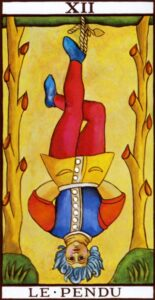
\includegraphics[scale=3]{a20220529HierarchicalOrderamongMankind-img001.jpg}
 \caption{The Hanged Man}
\end{wrapfigure}

In other words, the scientific approach does not require an inner transformation. Anyone, who is competent, can read the words and pass a multiple choice test, for example. Regarding esoteric knowledge, he explains:

\begin{quotex}
[it addresses] itself only to those people who are capable of the concentration and inner deepening necessary for intuition. … [it is] \textbf{a matter for an elite group of special people}.

\end{quotex}
He explains what that entails in \emph{Letter I: The Magician} in \emph{Meditations on the Tarot}:

\begin{quotex}
All practical esotericism is founded on the following rule: it is necessary to be one in oneself (\textbf{concentration without effort}) and one with the spiritual world (\textbf{to have a zone of silence in the soul}) in order for a revelatory or actual spiritual experience to be able to take place. In other words, if one wants to practise some form of authentic esotericism — be it mysticism, gnosis, or magic — it is necessary to be the Magician, i.e., concentrated without effort, operating with ease as if one were playing, and acting with perfect calm.

\end{quotex}
Those who are just reading the words, and they are beautiful, will be missing the most sublime meaning of the text. Unless the reader makes efforts toward inner transformation, starting with concentration and quelling the perturbations of the soul, he will miss the point. Tomberg explains that the book

\begin{quotex}
is written — and could only be written — for those who have the capacity and disposition to make use of the faculty of intuition as the direct sense for truth. Thus, it is addressed to those ``who have ears to hear and eyes to see.

\end{quotex}
\paragraph{Angelic Hierarchy}
Like Averroes, Tomberg recognizes that few people are able to experience the Divine Light in its fullness. The task of the angelic hierarchy, therefore, is to attenuate the Light in a manner appropriate to each one as it descends through the hierarchy. The esoteric path then is to reverse course and ascend through the hierarchy. To quote:

\begin{quotex}
Each lower rank of hierarchy is a ``moon" in relationship to the ``sun" of the rank above it.

The \textbf{angels} transmit the tumultuous, strong impulses of the \textbf{arch\-angels} in a bearable form, suited to human individuals, i.e., in the form of the soft light of moral clarity.

The \textbf{archangels} adopt the radical, valid-to-all-mankind commandments and prohibitions of the \textbf{principalities} (\emph{archai}) to suit the special characters and capacities of the various peoples, thereby protecting them from becoming over-pressured.

And something similar is effected by the \textbf{principalities} in relation to the \textbf{powers} (\emph{exusiai}), the \textbf{powers} toward the \textbf{virtues} (\emph{dynamis}), the virtues toward the \textbf{dominions} (\emph{kryriotetes}), the \textbf{dominions} toward the \textbf{thrones}, the \textbf{thrones} toward the \textbf{cherubim}, the \textbf{cherubim} toward the \textbf{seraphim}, and the \textbf{seraphim} toward the eternal \textbf{Trinity of God}.

\end{quotex}


\flrightit{Posted on 2022-05-29 by Cologero }

\begin{center}* * *\end{center}

\begin{footnotesize}\begin{sffamily}



\texttt{Jonathan Pageau on 2022-05-30 at 13:46 said: }

Hey Cologero. Reading the Meditations myself and thought of you. Hope you are well. Haven't connected in a long time.


\hfill

\texttt{Michael DeJoy on 2022-06-09 at 10:18 said: }

Concentration without effort requires the movement of energy. The areas of the thinking mind must be enlivened by the heart energy and the head energy acting together. When they are working together one finds the contentment they are looking for. The Magician will seem impossible as long as one is trying to figure it out, the ground must be established before that understanding is possible.


\hfill

\texttt{Cologero on 2022-06-09 at 14:34 said: }

Concentration is the ability to focus energy on one thing, which is the opposite of movement. Movement is due to automatic or mechanical thinking, i.e., the distraction arising from random thoughts that appears in consciousness.

As Tomberg explains:

``concentration is the willed silence of the automatism of the intellect and imagination"


\hfill

\texttt{Max on 2022-07-06 at 07:54 said: }

I am currently reading ``The Julian Jaynes Collection" to complement ``Origin of Consciousness". He has a useful analogy for understanding concentration: it is for the ``mind-space" what attention is for sense perception. It is especially difficult to realize when the mind-space is not even properly acknowledged in the first place, as is so common today. It evidently cannot be comprehended fundamentally by everyone.

What is agreeable with Jaynes is that he accepts this mind-space without too much reductionist baggage, even though he has some blind spots as well. In particular how mind-space is explained as a product of language, as if the name preceded the named. At any rate, here is an interesting quote on the topic:

``As the body with its sense organs (referred to as I) is to physical seeing, so there develops automatically an analog `I' to relate to this mental kind of `seeing' in mind-space. The analog `I' is the second most important feature of consciousness. It is not to be confused with the self, which is an object of consciousness in later development. The analog `I' is contentless, related I think to Kant's transcendental ego. As the bodily `I' can move about in its environment looking at this or that, so the analog `I' learns to `move about' in mind-space concentrating on one thing or another." -Jaynes

Of note is first that he seems to take the bodily I to be more ``real" than this analog `I'. That is obviously a prejudice which is not justified but taken for granted, since he subscribes to an evolutionary worldview. Secondly he describes its development process as ``automatic", which is merely another way of saying that he does not know. To be strict, automatic would mean that the I acts by itself, making it unreducible to anything else. Lastly, he says that concentration includes the capacity to move about in this mind-space without, conversely, letting it dominate us. 

Jaynes demonstrates, by his accurate descriptions from experience, that he knows concentration. That in itself makes him a more interesting author than the more scattered ones. He is aware of the important questions even though he does not have all the answers, which is an indispensable beginning.


\end{sffamily}\end{footnotesize}
